\section{All settings and robustness of the boundary}\label{app:ledger}

The certification boundary is stable: each of the 27 re-split settings (Tables~\ref{tab:dev_full} and~\ref{tab:mmlu_small_medium}) retains its outcome in at least 96\% of 200 re-drawn splits. At $\alpha=0.05$, none of the tested post-hoc alternative tests, scores, or learned predictors (Table~\ref{tab:sensitivity}) certifies a setting that ProbeMax rejects. Figure~\ref{fig:boundaries} shows every grid point of the large and small pairs, and Figure~\ref{fig:baselines} compares the policies with simple baselines under the same target. All grid tests are provided in the anonymous repository; gain retention and the label-light certificate are in Appendix~\ref{app:accuracy}, and boundary predictions in Appendix~\ref{app:predict}.

\begin{table}[!htbp]\centering\scriptsize
\caption{Ten of these 23 settings deploy and thirteen fall back (development). OLMo: large helper, OLMo-2-1124-7B-Instruct receiver; Llama: Llama-3.2-1B-Instruct helper, small receiver; Llama-8B: large helper, Llama-3.1-8B-Instruct receiver. Disagreements: $R$ and the reference answer differently; smallest 0.999 bound: smallest calibration Clopper--Pearson $0.999$ bound over the grid (diagnostic); fallback: no threshold passes; --: no question skipped; correct: development answers correct under the policy and under the reference. $^\ddagger$Nominal certificate (Appendix~\ref{app:history}). $^{*}$Without the 341 parser-review questions, only a lower $q$ is certified: 0.50 for medium/OBQA/C2C (47.8\% coverage, 7 of 355 changed), 0.50 for Llama-8B/OBQA, and 0.55 for Llama-8B/ARC. Parser-review questions: 341 calibration questions whose outputs were read with gold labels before the parser was frozen.}
\label{tab:dev_full}
\renewcommand{\arraystretch}{1.1}\setlength{\tabcolsep}{2.5pt}
\begin{tabular*}{\linewidth}{@{}lll@{\hspace{5pt}\extracolsep{\fill}}rccrccc@{}}\toprule
& & & \multicolumn{1}{c}{Disagreements} & & Smallest & Deployed & Coverage & Changed & Correct: policy\\
Pair & Task & Reference & \multicolumn{1}{c}{/ questions} & AUROC & 0.999 bound & \multicolumn{1}{c}{$q$} & (\%) & / skipped & / reference\\\midrule
small & OBQA & Text & 339/742 & 0.641 & 0.232 & fallback & 0.0 & -- & 346/346\\
small & OBQA & C2C & 350/742 & 0.700 & 0.161 & fallback & 0.0 & -- & 366/366\\
small & ARC & Text & 145/299 & 0.634 & 0.394 & fallback & 0.0 & -- & 126/126\\
small & ARC & C2C & 160/299 & 0.641 & 0.296 & fallback & 0.0 & -- & 155/155\\\midrule
medium & OBQA & Text & 174/742 & 0.787 & 0.096 & fallback & 0.0 & -- & 523/523\\
medium & OBQA & C2C$^{*}$ & 131/742 & 0.840 & 0.032 & 0.55 & 52.6 & 11/390 & 492/486\\
medium & ARC & Text & 52/299 & 0.742 & 0.102 & fallback & 0.0 & -- & 221/221\\
medium & ARC & C2C & 48/299 & 0.910 & 0.031 & 0.60 & 63.2 & 4/189 & 203/202\\\midrule
large & OBQA & Text$^\ddagger$ & 72/742 & 0.873 & 0.013 & 0.80 & 77.1 & 19/572 & 638/645\\
large & OBQA & C2C$^\ddagger$ & 60/742 & 0.883 & 0.016 & 0.80 & 77.1 & 13/572 & 605/598\\
large & ARC & Text & 15/299 & 0.952 & 0.019 & 0.95 & 95.0 & 9/284 & 270/274\\
large & ARC & C2C & 12/299 & 0.909 & 0.031 & 0.90 & 90.3 & 3/270 & 267/266\\
large & MMLU-Pro & Text & 561/2641 & 0.821 & 0.021 & 0.40 & 40.5 & 40/1069 & 1321/1319\\
large & MMLU-Pro & C2C & 756/2641 & 0.846 & 0.015 & 0.40 & 40.5 & 37/1069 & 1257/1233\\\midrule
OLMo & OBQA & Text & 172/742 & 0.790 & 0.118 & fallback & 0.0 & -- & 516/516\\
OLMo & ARC & Text & 67/299 & 0.749 & 0.169 & fallback & 0.0 & -- & 222/222\\
OLMo & MMLU-Pro & Text & 1112/2641 & 0.633 & 0.252 & fallback & 0.0 & -- & 664/664\\\midrule
Llama & OBQA & Text & 191/742 & 0.693 & 0.095 & fallback & 0.0 & -- & 333/333\\
Llama & OBQA & C2C & 427/742 & 0.618 & 0.325 & fallback & 0.0 & -- & 358/358\\
Llama & ARC & Text & 88/299 & 0.678 & 0.296 & fallback & 0.0 & -- & 145/145\\
Llama & ARC & C2C & 174/299 & 0.615 & 0.247 & fallback & 0.0 & -- & 146/146\\\midrule
Llama-8B & OBQA & Text$^{*}$ & 86/742 & 0.874 & 0.022 & 0.60 & 59.0 & 7/438 & 638/636\\
Llama-8B & ARC & Text$^{*}$ & 37/299 & 0.880 & 0.033 & 0.70 & 68.9 & 4/206 & 258/260\\
\bottomrule
\end{tabular*}
\end{table}

\paragraph{Calibration statistics.} Table~\ref{tab:calstats} lists the calibration test at the deployed quantile for the 14 OBQA, ARC, and large-pair MMLU-Pro settings (Table~\ref{tab:dev_full}), or at the grid point with the smallest $p$-value for fallbacks. With $\alpha=0.05$ and $\delta=0.001$, a skipped subset with no observed changes passes only if it contains at least 135 calibration questions, since $0.95^{135}<0.001<0.95^{134}$. At $q=0.05$, the small pair skips only 65 OBQA and 18 ARC calibration questions. Figure~\ref{fig:boundaries} shows the full grid: the large pair's 0.999 upper bound stays below 5\% until 78 to 94\% of calibration questions are skipped, whereas the small pair's never falls below 16\%.

\begin{table}[!htbp]\centering\scriptsize
\caption{Deployed settings pass the exact test with 290 to 2,358 skipped calibration questions, whereas the small pair's best candidates skip at most 65. Rows: small, medium, and large pairs only. Tested $q$: the deployed quantile, or for a fallback the grid point with the smallest $p$; $n$, $k$: skipped and changed calibration questions at the tested $q$; $p$: exact-test p-value; --: not applicable. Reviewed out: the test without the 341 parser-review questions. Parser-review questions: 341 calibration questions whose outputs were read with gold labels before the parser was frozen (none on MMLU-Pro). Re-split: share of 200 re-drawn splits that deploy. Needed $N_{\rm cal}$: calibration size at which the observed rate would pass (never: the observed rate is at least 0.05). $^\ddagger$Nominal certificate (Text: reused from an earlier 100-test family; Appendix~\ref{app:history}).}
\label{tab:calstats}
\renewcommand{\arraystretch}{1.1}\setlength{\tabcolsep}{2.5pt}
\begin{tabular*}{\linewidth}{@{}lll@{\hspace{5pt}\extracolsep{\fill}}ccccccccc@{}}\toprule
& & & & & \multicolumn{3}{c}{Full calibration split} & \multicolumn{2}{c}{Reviewed out} & & \\\cmidrule(lr){6-8}\cmidrule(lr){9-10}
Pair & Task & Reference & Deployed $q$ & Tested $q$ & $n$ & $k$ & $p$ & $k/n$ & $p$ & Re-split & Needed $N_{\rm cal}$\\\midrule
small & OBQA & Text & fallback & 0.05 & 65 & 5 & 0.894 & -- & -- & 0.00 & never\\
small & OBQA & C2C & fallback & 0.05 & 65 & 2 & 0.363 & -- & -- & 0.00 & 21,793\\
small & ARC & Text & fallback & 0.10 & 33 & 5 & 0.995 & -- & -- & 0.00 & never\\
small & ARC & C2C & fallback & 0.10 & 33 & 2 & 0.773 & -- & -- & 0.00 & never\\
\addlinespace[2pt]
medium & OBQA & Text & fallback & 0.05 & 601 & 36 & 0.884 & -- & -- & 0.00 & never\\
medium & OBQA & C2C & 0.55 & 0.55 & 739 & 19 & $6.9\times10^{-4}$ & 18/640 & $4.4\times10^{-3}$ & 1.00 & --\\
medium & ARC & Text & fallback & 0.05 & 256 & 12 & 0.483 & -- & -- & 0.00 & 79,333\\
medium & ARC & C2C & 0.60 & 0.60 & 290 & 1 & $5.6\times10^{-6}$ & 1/210 & $2.5\times10^{-4}$ & 0.96 & --\\
\addlinespace[2pt]
large & OBQA & Text$^\ddagger$ & 0.80 & 0.80 & 1064 & 18 & $1.2\times10^{-8}$ & 17/908 & $7.8\times10^{-7}$ & 1.00 & --\\
large & OBQA & C2C$^\ddagger$ & 0.80 & 0.80 & 1064 & 22 & $6.7\times10^{-7}$ & 19/908 & $5.4\times10^{-6}$ & 1.00 & --\\
large & ARC & Text & 0.95 & 0.95 & 422 & 4 & $4.8\times10^{-6}$ & 2/297 & $3.4\times10^{-5}$ & 1.00 & --\\
large & ARC & C2C & 0.90 & 0.90 & 404 & 7 & $5.4\times10^{-4}$ & 2/282 & $6.6\times10^{-5}$ & 1.00 & --\\
large & MMLU-Pro & Text & 0.40 & 0.40 & 2358 & 67 & $1.3\times10^{-7}$ & 67/2358 & $1.3\times10^{-7}$ & 1.00 & --\\
large & MMLU-Pro & C2C & 0.40 & 0.40 & 2358 & 75 & $1.0\times10^{-5}$ & 75/2358 & $1.0\times10^{-5}$ & 1.00 & --\\\bottomrule
\end{tabular*}
\end{table}

\begin{figure}[!t]\centering
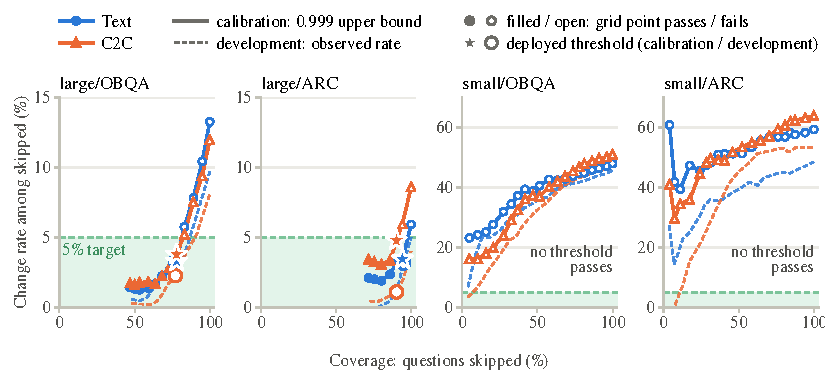
\includegraphics[width=\linewidth]{figures/figure_boundaries.pdf}
\caption{The large pair passes the test over a wide range of thresholds under both references, whereas no threshold passes for the small pair. Each curve runs over the 20 predetermined quantiles of the same ProbeMax score, plotted against the share of questions skipped on its own population. Solid: calibration Clopper--Pearson $0.999$ upper bound on the change rate among skipped questions; a grid point passes the exact test ($p\le0.001$) exactly when this bound is below the 5\% target (green band; filled markers). Dashed: observed change rate among skipped development questions, which does not certify a threshold. Star and ring: deployed threshold on calibration and development. Low quantiles that share the zero threshold coincide. Vertical ranges differ by pair; medium-pair summaries are in Table~\ref{tab:dev_full}. Both large/OBQA certificates are nominal (Appendix~\ref{app:history}).}
\label{fig:boundaries}
\end{figure}

\paragraph{Stability and sensitivity.} We re-drew the fit and calibration splits of these 27 settings 200 times using the original grouping, sizes, and shuffle rule (for MMLU-Pro, the seed of its fixed pseudorandom order), recomputed the 20 thresholds, and reran the test; development sets remained unchanged. Medium/ARC/C2C deploys in 96\% of re-draws, every other deployment in all 200, and no fallback setting deploys in any (the stronger-helper fallbacks certify in none and 15.5\%, Appendix~\ref{app:informed}; Text+fact and GSM8K were not re-split). Among deploying re-draws, the median deployed $q$ matches the original everywhere except large/ARC/Text (0.90 instead of 0.95). Five fallback settings observe a change rate below 0.05 but would need 3,975 (OLMo/ARC/Text), 7,494 (Llama/OBQA/Text), 13,386 (Llama/ARC/C2C), 21,793 (small/OBQA/C2C), and 79,333 (medium/ARC/Text) calibration questions to pass. The medium pair's disagreement remains similar across its fit, calibration, and development splits (OBQA: 24.4, 25.5, and 23.5\% with Text, 16.8, 17.7, and 17.7\% with C2C; ARC: 20.0, 15.0, and 17.4\%, and 16.0, 12.3, and 16.1\%), and its probe produced no \textsc{invalid} score.

\paragraph{Post-hoc variants.} Table~\ref{tab:sensitivity} recomputes every setting from saved records under post-hoc variants modifying one element each. The variants are: setting $\alpha=0.02$ or $0.10$ with the same per-candidate cutoff; fixed-sequence testing (evaluating candidates in ascending order of $q$, each at the family's 0.02 Bonferroni bound instead of 0.001, deploying the last accepted $q$); replacing ProbeMax with probe entropy or one minus the top-two probability margin (read from the same prefill); and using the learned predictor below. This predictor is refitted per setting on its fit split using historical features and hyperparameters (fixed on large/OBQA/Text, not tuned per setting). Thresholds always derive from fit-split quantiles. At $\alpha=0.05$, no variant certifies a setting that ProbeMax rejects, and every small-pair setting falls back under all variants. Setting $\alpha=0.02$ removes the medium pair, large/ARC/C2C, and MMLU-Pro/Text, while $\alpha=0.10$ adds medium/OBQA/Text. Fixed receiver-only execution ($q=1$), which fails the prespecified test everywhere, is accepted for large-pair ARC at $\alpha=0.10$ (both references) and under fixed-sequence testing (Text; 12 changes among 448 calibration questions, $p=0.011$). The learned predictor's development AUROC for receiver--reference disagreement trails ProbeMax's in every setting (0.55--0.64 for the small pair, 0.69--0.75 for the medium pair, 0.64--0.88 for the large pair); its lower coverage does not imply learned skipping is useless. Fixed-sequence testing yields an equal or larger $q$ across all settings here, but it depends on testing order and stops at the first failure. Bonferroni remains primary because it was prespecified before choosing these variants.

\begin{table}[!htbp]\centering\scriptsize
\caption{At $\alpha=0.05$, no post-hoc variant certifies a setting that the prespecified procedure rejects. (a) Deployed $q$, the quantile that sets the skip threshold (a larger $q$ skips more questions, and 1 skips all); --: no threshold passes, so the setting keeps communicating (fallback). (b) At the deployed $q$, skipped development questions whose answer changes, out of all skipped ones. Primary: ProbeMax, $\alpha=0.05$, $\delta=0.001$. Row small/both/both: the four small-pair OBQA and ARC settings. Fixed sequence: candidates tested in ascending order of $q$, each at 0.02 instead of 0.001, until one fails. Entropy, Margin: probe entropy, or one minus the top-two probability margin, replaces ProbeMax. Learned: learned predictor (receiver hidden-state logistic regression refitted on each fit split). $^\ddagger$Nominal certificate (Text: reused from an earlier 100-test family; Appendix~\ref{app:history}); $^\S$tested on its calibration labels before.}
\label{tab:sensitivity}
\renewcommand{\arraystretch}{1.2}\setlength{\tabcolsep}{3pt}
\vspace{5pt}\textit{(a) Deployed $q$}\par\smallskip
\begin{tabular*}{\linewidth}{@{}lll@{\extracolsep{\fill}}ccccccc@{}}\toprule
& & & & \multicolumn{6}{c}{Post-hoc variants}\\\cmidrule(l){5-10}
Pair & Task & Reference & Primary & $\alpha=0.02$ & $\alpha=0.10$ & Fixed sequence & Entropy & Margin & Learned\\\midrule
small & both & both & -- & -- & -- & -- & -- & -- & --\\
\addlinespace[3pt]
medium & OBQA & Text & -- & -- & 0.45 & -- & -- & -- & --\\
medium & OBQA & C2C & 0.55 & -- & 0.65 & 0.55 & 0.55 & 0.55 & --\\
medium & ARC & Text & -- & -- & -- & -- & -- & -- & --\\
medium & ARC & C2C & 0.60 & -- & 0.75 & 0.60 & 0.60 & 0.60 & --\\
\addlinespace[3pt]
large & OBQA & Text$^\ddagger$ & 0.80 & 0.65 & 0.90 & 0.80 & 0.80\rlap{$^\S$} & 0.80 & 0.30\rlap{$^\S$}\\
large & OBQA & C2C$^\ddagger$ & 0.80 & 0.65 & 0.95 & 0.85 & 0.80 & 0.80 & 0.55\\
large & ARC & Text & 0.95 & 0.80 & 1 & 1 & 0.95 & 0.95 & 0.90\\
large & ARC & C2C & 0.90 & -- & 1 & 0.95 & 0.90 & 0.90 & 0.65\\
large & MMLU-Pro & Text & 0.40 & -- & 0.60 & 0.45 & 0.40 & 0.40 & 0.05\\
large & MMLU-Pro & C2C & 0.40 & 0.25 & 0.50 & 0.40 & 0.40 & 0.40 & --\\\bottomrule
\end{tabular*}
\par\vspace{17pt}
\textit{(b) Changed / skipped development questions at the deployed $q$}\par\smallskip
\begin{tabular*}{\linewidth}{@{}lll@{\extracolsep{\fill}}ccccccc@{}}\toprule
& & & & \multicolumn{6}{c}{Post-hoc variants}\\\cmidrule(l){5-10}
Pair & Task & Reference & Primary & $\alpha=0.02$ & $\alpha=0.10$ & Fixed sequence & Entropy & Margin & Learned\\\midrule
small & both & both & -- & -- & -- & -- & -- & -- & --\\
\addlinespace[3pt]
medium & OBQA & Text & -- & -- & 18/321 & -- & -- & -- & --\\
medium & OBQA & C2C & 11/390 & -- & 25/481 & 11/390 & 11/389 & 11/391 & --\\
medium & ARC & Text & -- & -- & -- & -- & -- & -- & --\\
medium & ARC & C2C & 4/189 & -- & 7/219 & 4/189 & 3/187 & 3/187 & --\\
\addlinespace[3pt]
large & OBQA & Text$^\ddagger$ & 19/572 & 6/460 & 44/676 & 19/572 & 18/572 & 19/572 & 6/230\\
large & OBQA & C2C$^\ddagger$ & 13/572 & 1/460 & 45/703 & 22/613 & 13/572 & 13/572 & 13/399\\
large & ARC & Text & 9/284 & 0/233 & 15/299 & 15/299 & 9/284 & 9/284 & 7/272\\
large & ARC & C2C & 3/270 & -- & 12/299 & 6/284 & 3/270 & 3/270 & 4/194\\
large & MMLU-Pro & Text & 40/1069 & -- & 109/1596 & 56/1205 & 40/1068 & 40/1069 & 5/128\\
large & MMLU-Pro & C2C & 37/1069 & 6/697 & 85/1341 & 37/1069 & 37/1068 & 38/1069 & --\\\bottomrule
\end{tabular*}
\end{table}

\paragraph{Same-target baselines (post hoc).} Figure~\ref{fig:baselines} compares each policy with two simple skipping baselines under the same target; no threshold, reference, or split was changed, and neither baseline was replayed end-to-end. Fixed receiver-only execution ($q=1$) fails the test in all 14 OBQA, ARC, and large-pair MMLU-Pro settings (calibration change rate 2.7 to 56.7\%). The two large-pair ARC rates fall below 5\% but yield $p=0.011$ (Text, 12 of 448) and $p=0.435$ (C2C, 21 of 448); there, fixed $R$ answers about as many development questions correctly as the certified policies, at a lower component-estimated latency. A rule skipping questions at random, independently of content, changes answers at the receiver--reference disagreement rate in expectation regardless of coverage (2.7 to 29.1\% on calibration for the eight deployed settings). At the policy's development coverage $\kappa$, its expected correct count $(1-\kappa)\,a_b+\kappa\,a_R$ (where $a_b$ and $a_R$ are the correct counts of the reference and $R$) exceeds the policy's in three C2C settings (medium ARC, large OBQA, large ARC) and trails it in the other five. Its component-estimated latency is 18 to 67~ms lower (it runs no probe, and its decision overhead was not measured). The probability that a random subset of a grid point's size, drawn without replacement from the fixed calibration split, passes the test remains below $10^{-4}$ at every grid point in every setting except large ARC with Text, peaking at 0.017 (at $q=0.80$). These are per-grid-point probabilities, not the probability that a search over the grid passes.

\begin{figure}[!t]\centering
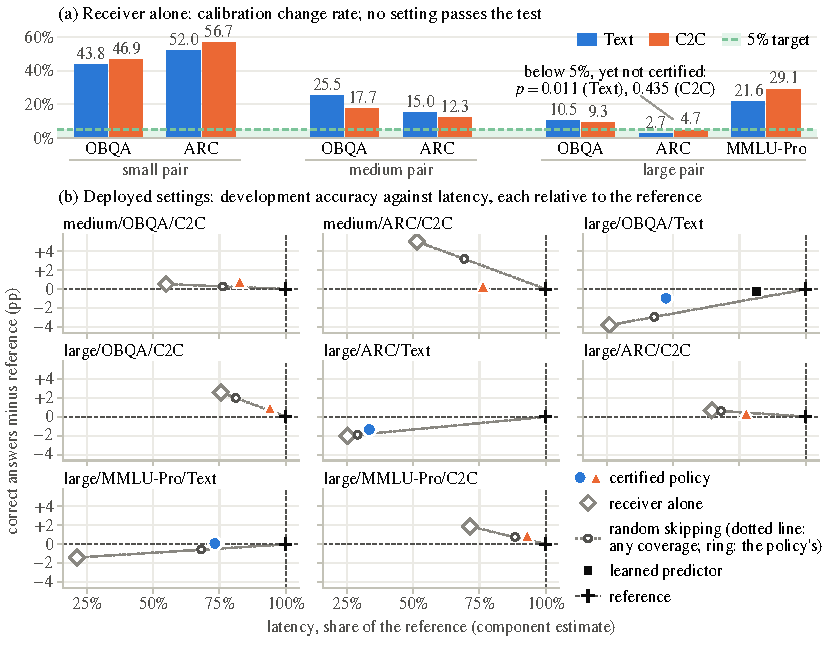
\includegraphics[width=\linewidth]{figures/figure_baselines.pdf}
\caption{Receiver-alone execution fails the test everywhere and random skipping carries no certificate, although both can answer as well as the certified policy or run faster. (a)~Fixed receiver-only execution: calibration change rate in the 14 OBQA, ARC, and large-pair MMLU-Pro settings; none passes the test, including the two large-pair ARC settings below the 5\% target (green band; $p$: exact-test p-value). (b)~The eight deployed settings, one panel each, in the accuracy--latency plane relative to the fixed reference ($+$, dashed lines). Horizontal: mean latency as a share of the reference's, recomposed from per-question development latencies (component estimates, not end-to-end measurements); the policy includes its probe, and random skipping has none. Vertical: development correct answers minus the reference, in percentage points. Filled circle or triangle: the certified policy (Text or C2C); open diamond: receiver alone; dotted line: random skipping at any coverage, which lies on the line from receiver alone to the reference, with a ring at the policy's coverage (expected count); black square: the historical learned predictor (large/OBQA/Text), an earlier stage's receiver hidden-state logistic regression, at its latency in that stage's accounting.}
\label{fig:baselines}
\end{figure}

\paragraph{Historical learned predictor.} An earlier stage evaluated ProbeMax and a learned predictor on large/OBQA/Text using the same grid, $\alpha$, and cutoff, within its declared 100-test family (Bonferroni level 0.10; Appendix~\ref{app:history}), where both passed. The predictor is an L2-regularized logistic regression on 8,192-dimensional receiver hidden states (last-token outputs of an intermediate layer and the final normalization layer of Qwen3-8B), fitted on the 2,100 fit questions to predict receiver--Text disagreement. It requires reference executions and offline feature extraction but no correctness labels. It skipped 230 of 742 development questions with 6 changes and 643 correct answers (component latency 797.2~ms in that stage's accounting), against 572 skipped, 19 changes, 638 correct, and 460.9~ms for ProbeMax (462.9~ms in the unified records of Figure~\ref{fig:baselines}).

\begin{table}[!htbp]\centering\scriptsize
\caption{All four small- and medium-pair MMLU-Pro settings fall back, and none certifies in any of 200 re-drawn splits ($N=2641$ development questions). Disagreement: share of development questions on which $R$ and the reference answer differently. Best candidate: smallest exact-test p-value over the 20 candidates, with its $k/n$ (changed/skipped calibration questions). Correct and \textsc{invalid}: development counts of $R$ and the reference. Re-split: share of the 200 re-drawn splits that deploy.}
\label{tab:mmlu_small_medium}
\renewcommand{\arraystretch}{1.1}\setlength{\tabcolsep}{2.5pt}
\begin{tabular*}{\linewidth}{@{}ll@{\hspace{5pt}\extracolsep{\fill}}cccccccccc@{}}\toprule
& & & & \multicolumn{2}{c}{Best candidate} & & \multicolumn{2}{c}{Correct} & \multicolumn{2}{c}{\textsc{invalid}} & \\\cmidrule(lr){5-6}\cmidrule(lr){8-9}\cmidrule(lr){10-11}
Pair & Reference & Disagreement (\%) & AUROC & $p$ & $k/n$ & Deployed $q$ & $R$ & Reference & $R$ & Reference & Re-split\\\midrule
small & Text & 46.76 & 0.644 & 1 & 102/280 & fallback & 403 & 516 & 151 & 229 & 0.000\\
small & C2C & 60.24 & 0.626 & 1 & 106/280 & fallback & 403 & 462 & 151 & 420 & 0.000\\
medium & Text & 42.71 & 0.717 & 1 & 64/690 & fallback & 813 & 913 & 160 & 18 & 0.000\\
medium & C2C & 53.39 & 0.765 & 0.193 & 29/690 & fallback & 813 & 530 & 160 & 1124 & 0.000\\\bottomrule
\end{tabular*}
\end{table}

\begin{table}[!htbp]\centering\scriptsize
\caption{The pooled MMLU-Pro certificate gives no subgroup guarantee: some categories exceed 5\% changed answers (development group representatives; descriptive). Both references skip the same questions. Policy: large pair at its deployed $q$; $N$: development questions in the category.}
\label{tab:mmlu_subgroups}
\begin{tabular*}{\linewidth}{@{}l@{\extracolsep{\fill}}rcccc@{}}\toprule
& & & & \multicolumn{2}{c@{}}{Changed / skipped}\\\cmidrule(l){5-6}
Category & \multicolumn{1}{c}{$N$} & Skipped & Coverage (\%) & Text & \multicolumn{1}{c@{}}{C2C}\\\midrule
biology & 144 & 100 & 69.4 & 1/100 & 0/100\\
business & 177 & 47 & 26.6 & 1/47 & 2/47\\
chemistry & 257 & 60 & 23.3 & 4/60 & 6/60\\
computer science & 93 & 42 & 45.2 & 4/42 & 1/42\\
economics & 190 & 116 & 61.1 & 2/116 & 0/116\\
engineering & 220 & 72 & 32.7 & 4/72 & 12/72\\
health & 155 & 95 & 61.3 & 5/95 & 0/95\\
history & 86 & 47 & 54.7 & 1/47 & 0/47\\
law & 217 & 62 & 28.6 & 4/62 & 2/62\\
math & 305 & 97 & 31.8 & 4/97 & 9/97\\
other & 210 & 96 & 45.7 & 5/96 & 1/96\\
philosophy & 113 & 39 & 34.5 & 2/39 & 0/39\\
physics & 293 & 82 & 28.0 & 0/82 & 3/82\\
psychology & 181 & 114 & 63.0 & 3/114 & 1/114\\
\bottomrule\end{tabular*}
\end{table}

\paragraph{MMLU-Pro.}\label{app:mmlu} The large receiver shows exact zero uncertainty on 713 of 3,000 fit groups (1,442 of 6,000 calibration groups), merging quantiles $q\le0.20$ into one threshold. Both large-pair references pass at $q=0.40$ (67 and 75 changes among 2,358 skipped calibration groups) and fail at $q=0.45$ (105 and 118 of 2,654; $p=0.0063$ and $0.101$). On development, ProbeMax's average precision for disagreement is 0.522 (Text) and 0.629 (C2C). Of the policies' changed answers, 14 (Text) and 27 (C2C) became correct, 12 and 3 became incorrect, and 14 and 7 stayed incorrect. \textsc{invalid} counts are 6 ($R$), 2 (Text), and 20 (C2C), and 2 and 19 for the two policies. The pooled certificate gives no subgroup guarantee: some development categories exceed 5\% changed answers (e.g., engineering C2C, 12 of 72; Table~\ref{tab:mmlu_subgroups}). Run within each of the 14 categories under a rule fixed before computing, using category-specific fit quantiles and calibration questions, the test certifies three categories for Text (biology, economics, and engineering; the latter changing 5 of 102 skipped development answers under its own threshold) and three for C2C (health, other, and psychology). With $\delta$ further divided by 14, it certifies none for Text and one (psychology) for C2C. All four small- and medium-pair settings fall back (smallest $p=0.193$ over 80 tests; disagreement 42.7 to 60.2\%, AUROC 0.626 to 0.765; Table~\ref{tab:mmlu_small_medium}). Their answers fail to parse more often, above all with C2C: \textsc{invalid} shares of development answers are 5.7 ($R$), 8.7 (Text), and 15.9\% (C2C) for the small pair, and 6.1, 0.7, and 42.6\% for the medium pair, compared to 0.2, 0.1, and 0.8\% for the large pair. Consequently, medium-pair C2C answers far fewer questions correctly than the receiver alone (530 against 813). Their three-action headroom is 11.59 (small) and 7.91 points (medium) over the best fixed action, against 9.05 for the large pair, and 15.87 and 11.70 points over the receiver alone (no null control was run for them).

